\section{Test af accelerometer} 
\label{sec:test_acc}
I dette projekt anvendes to accelerometer som sensorer til opsamling af signaler. For at kunne anvende et accelerometer er det vigtigt at kende forskellige tolerancer i forhold til deres datablade, hvorfor et forsøg udføres for at kunne tage højde for disse parametre.

\subsection{Formål}
Denne test har til formål at identificere spændingen i henholdsvis $0^{\circ}$ og $90^{\circ}$, hvorudfra vinkler kan beregnes. Derudover identificeres støjsignaler i outputsignalet samt offsettet og sensitiviteten, så dette kan tages højde for i pilotforsøget \autoref{sec:pilotforsoeg} og senere forsøg.

\begin{enumerate}
\item Identificering af spænding ved $0^{\circ}$ og $90^{\circ}$
\item Identificering af støj i outputsignaler for accelerometrene
\item Identificering af offsettet og sensitiviteten for accelerometrene
\end{enumerate}

\subsection{Materialer}
\begin{itemize}
\item Accelerometre ADXL$335$
\item Tape
\item Vinkel
\item Vaterpas
\item Breadboard
\item Computer med Scopelogger og MATLAB
\item NI USB-6009
\end{itemize}

\subsection{Metode}
Alle målingerne er foretaget i alle tre retninger. 
\begin{enumerate}
\item Der foretages målinger ved $0$ g-påvirkning, hvilket svarer til en hældning på $0^{\circ}$ og ved $1$ g-påvirkning, hvilket svarer til en hældning på $90^{\circ}$
\item Støjsignaler i outputtet identificeres ved måling af baseline uden nogen g-påvirkningen, hvorefter det måles ved $1$ g-påvirkningen. 
\item På baggrund af de forrige mål kan offsettet og sensitiviteten udregnes
\end{enumerate}

\subsection{Forsøgsopstilling}
Forsøgsopstillingen udføres på samme måde for begge accelerometre.
\begin{itemize}
\item Accelerometeret tilkobles breadboard og sættes fast med tape.
\item Accelerometeret indstilles så det er vinkelret
\begin{itemize}
\item Accelerometeret placeres efter fremgangsmåden \autoref{sec:acc_fremgangsmaade}
\end{itemize}
\item Accelerometeret tilkobles NI USB-6009
\item NI USB-6009 tilkobles computer
\end{itemize}

\subsection{Fremgangsmåde} 
\label{sec:acc_fremgangsmaade}
Der foretages 6 forskellige målinger for hvert accelerometer. Fremgangsmåden er illustreret på \autoref{fig:acc1} og \autoref{fig:acc2}
\begin{itemize}
\item Accelerometeret er plan på bordet opad
\item Accelerometeret er plan på bordet nedad
\item Accelerometeret er lodret opad
\item Accelerometeret er lodret nedad
\item Accelerometeret er vandret mod højre
\item Accelerometeret er vandret mod venstre
\end{itemize}


\begin{figure}[H]
\centering
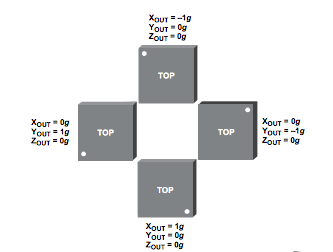
\includegraphics[width=0.3\textwidth]{figures/acc1}
\caption{Påvirkning af accelerometeret i lodret og vandret position \citep{analogdevices2010}}
\label{fig:acc1}
\end{figure}


\begin{figure}[H]
\centering
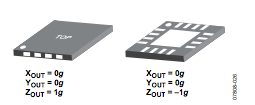
\includegraphics[width=0.3\textwidth]{figures/acc2}
\caption{Påvirkning af accelerometeret i plan \citep{analogdevices2010}}
\label{fig:acc2}
\end{figure}

